\documentclass[Rapport/Playerside/GameController/GameController.tex]{subfiles}
\label{sec:playerside_GameController_design}
\begin{document}
\subsubsection{Design}
I dette afsnit beskrives design for GameController klassen på PlayerSideApp. Denne klasse er controller klassen for PlayerSideApp, og indeholder alt den logik, der skal til, for at de 3 boundary klasser RPI\_IF, CupSensor\_IF og CupLight\_IF fungerer i et samlet system. Under designet af denne klasse har det været vigtigt at følge sekvensdiagrammet og statediagram i arkitekturet og bruge de funktioner, der har været defineret i de forskellige boundaryklasser. En del af designet af klassen bestod i også alt lave stubs for funktionerne i de 3 boundaryklasser, så det eneste der skulle gøres i en videre integrering  var at slette implementeringen af stubs og bruge de rigtige funktioner. UART er generelt brugt rigtig meget til at udskrive information om de forskellige funktioner. På denne måde var systemet let at debugge. En funktion i gamecontrolleren, der er interessant at snakke om er blinkefunktionen i systemet, som denne klasse skal styre. Her bliver en timer i PSoC komponent kataloget brugt. Denne komponent startes og stoppes i klassens Controller funktion. Når timeren startes skal den interrupte hvert halve sekund. Her bliver funktionen interrupt\_blink brugt i dens interruptvektor, der skal kontrollere de 6 LED'er, når de  skal blinke. Timer komponenten brugt kan ses i figur \ref{fig:Timer}.
\begin{figure}
    \centering 
    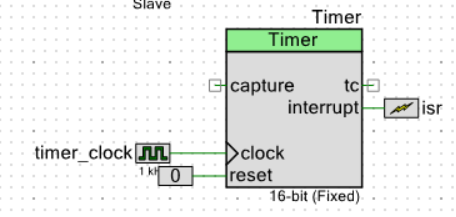
\includegraphics[width=0.5\linewidth]{Softwaredesign/GameController/graphic/gamecontroller_timer.PNG}
    \caption{Timer brugt til implementering af blink funktion}
    \label{fig:Timer}
\end{figure}
For en mere uddybende beskrivelse af design for GameController klassen, heri de forskellige funktioner, så se afsnit \fullref{sec:GameController_design_bilag} i bilaget.
\end{document}
